\documentclass{article}

\usepackage{graphicx}
\usepackage{tikz}
\usepackage{tikzsymbols}
\usetikzlibrary{calc,patterns,shapes.geometric}
\pagestyle{empty}
\usepackage[margin=0pt]{geometry}
\geometry{papersize={14in,12in}}

\def\centerarc[#1](#2)(#3:#4:#5){\draw[#1] ($(#2)+({#5*cos(#3)},{#5*sin(#3)})$) arc (#3:#4:#5);}

\begin{document}
	\begin{figure}
		\centering
		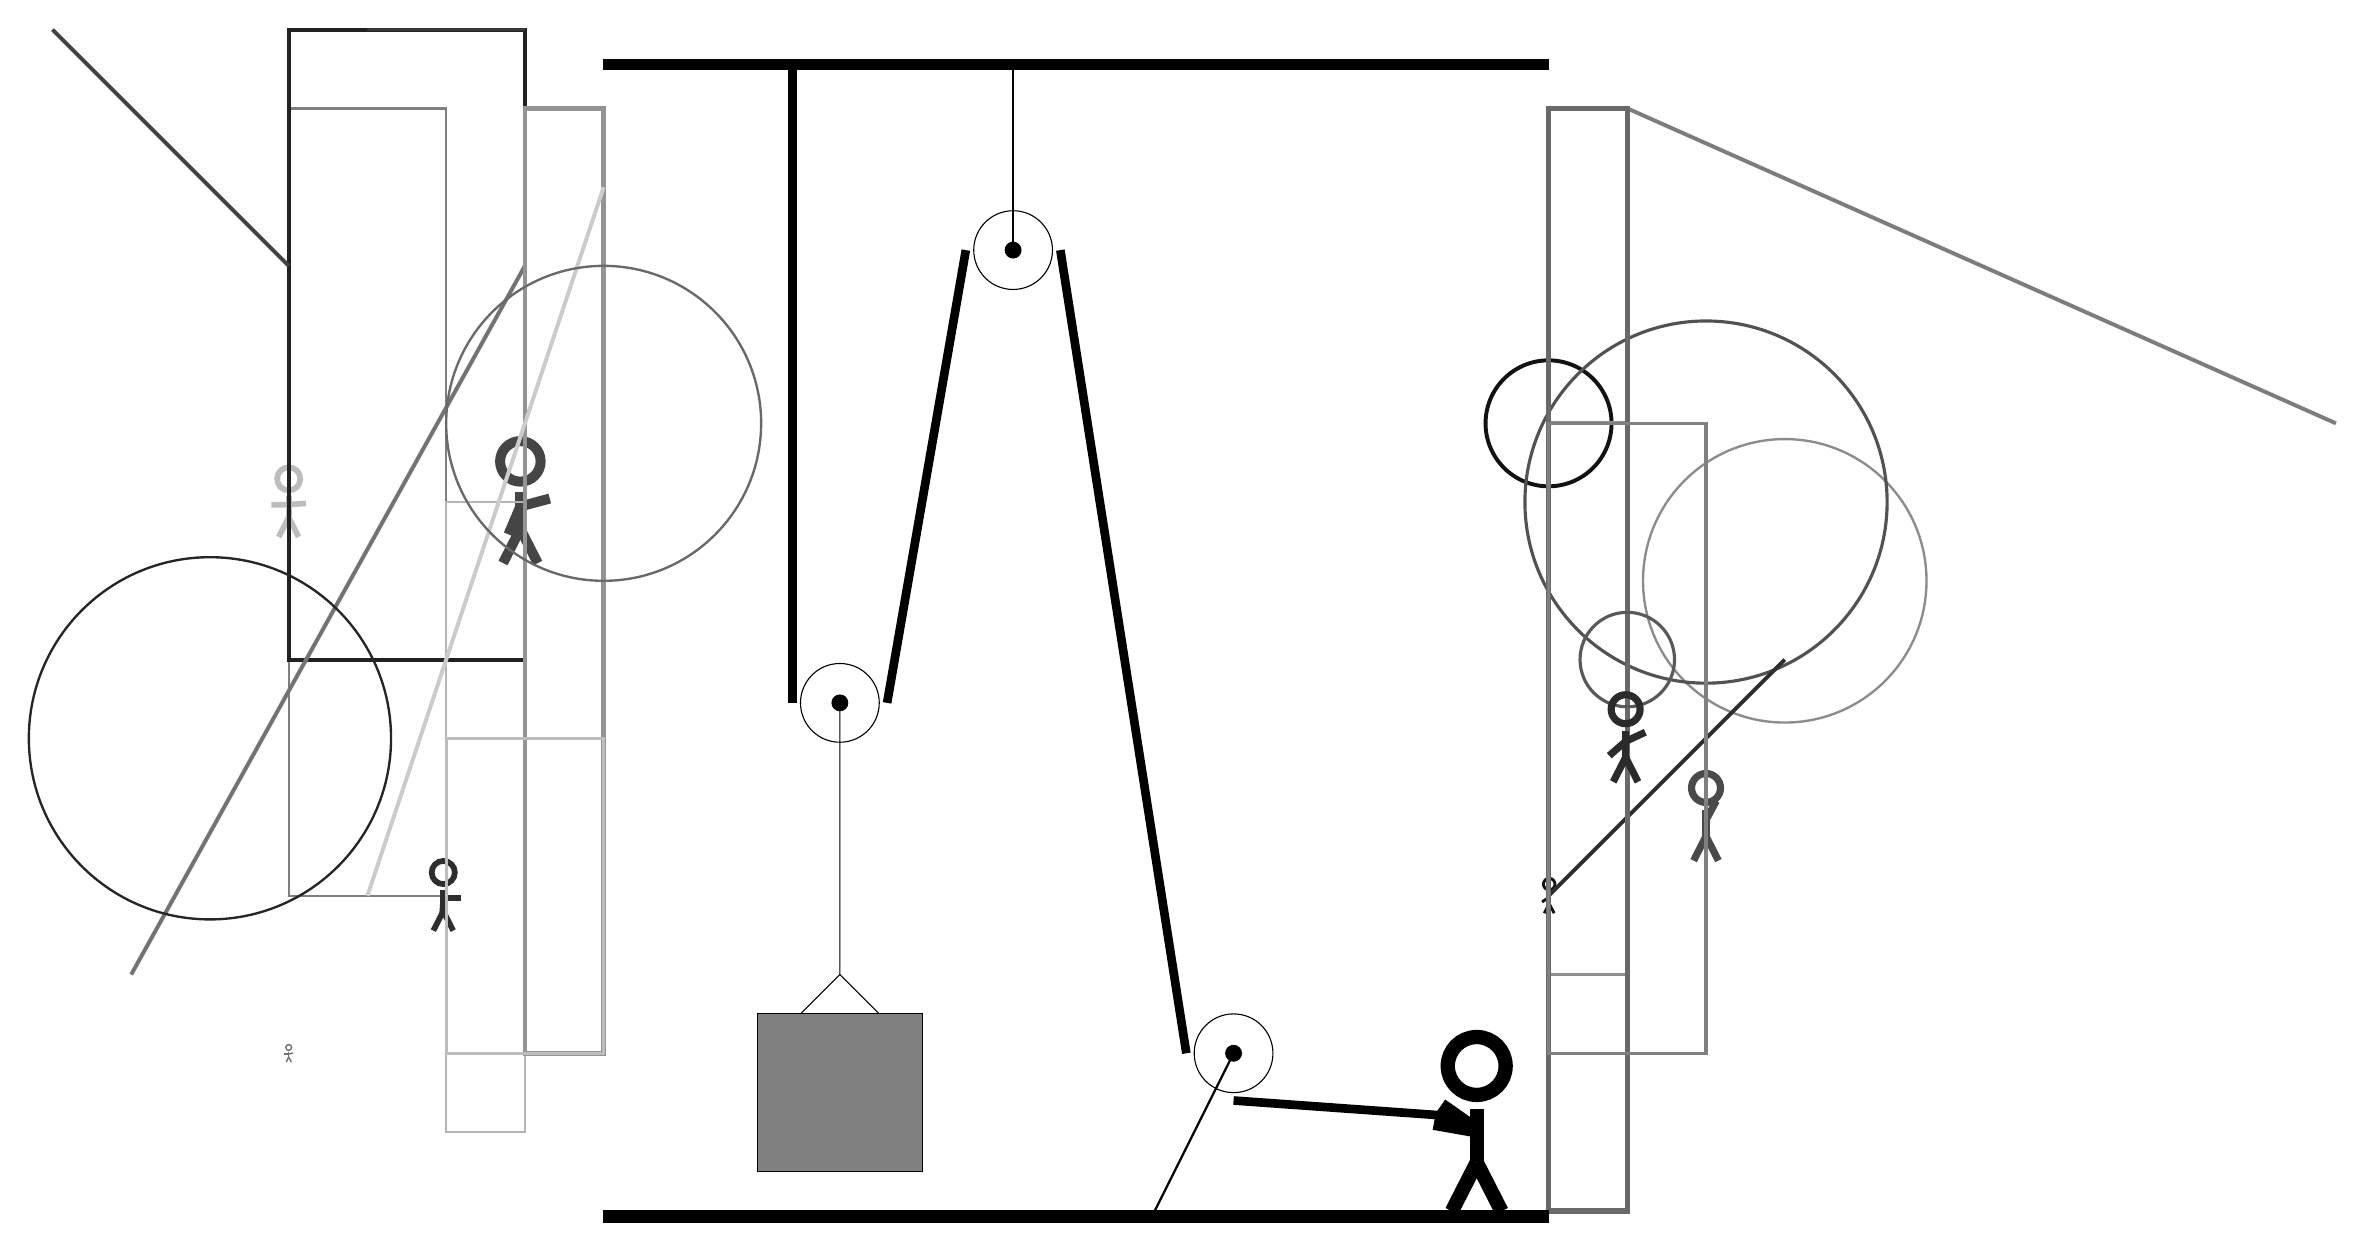
\begin{tikzpicture}
			%%%%% START %%%%%
			
			\draw[fill=black] (-2, 11.5) rectangle (10, 11.625);
			
			\draw[line width=0.5mm, color=black!52](-2, 7) -- (-2, 7);
			
			\node[line width=0.7mm, color=black!26] at (-6, 6) {\Strichmaxerl[4][1][4]};
			\draw[line width=0.3mm, color=black!50] (-4, 11) rectangle (-6, 1);
			\draw[line width=0.5mm, color=black!87] (-3, 12) rectangle (-6, 4);
			\draw[line width=0.5mm, color=black!55](-3, 9) -- (-8, 0);
			\node[line width=0.4mm, color=black!73] at (-3, 6) {\Strichmaxerl[7][67][15]};
			\node[line width=0.7mm, color=black!71] at (12, 2) {\Strichmaxerl[5][89][62]};
			\draw [line width=0.5mm, color=black!93](10, 7) circle (0.8);
			\node[line width=0.2mm, color=black!56] at (-6, -1) {\Strichmaxerl[1][0][10]};
			
			\draw [line width=0.3mm, color=black!45](13, 5) circle (1.8);
			
			\draw [line width=0.4mm, color=black!28](15, 4) circle (0.0);
			\draw[line width=0.3mm, color=black!29] (-4, 6) rectangle (-3, -2);
			\draw[line width=0.6mm, color=black!42] (-3, -1) rectangle (-2, 11);
			\node[line width=0.5mm, color=black!82] at (-4, 1) {\Strichmaxerl[4][86][0]};
			\draw[line width=0.5mm, color=black!51](11, 11) -- (20, 7);
			\draw[line width=0.5mm, color=black!44] (10, 7) rectangle (11, 0);
			
			\draw[line width=0.5mm, color=black!74](-6, 9) -- (-9, 12);
			\draw [line width=0.4mm, color=black!68](12, 6) circle (2.3);
			\node[line width=0.5mm, color=black!93] at (10, 1) {\Strichmaxerl[2][35][72]};
			
			\draw[line width=0.5mm, color=black!82](13, 4) -- (10, 1);
			\draw[line width=0.5mm, color=black!20](-2, 10) -- (-5, 1);
			
			\draw [line width=0.3mm, color=black!85](-7, 3) circle (2.3);
			\draw[line width=0.7mm, color=black!59] (10, -3) rectangle (11, 11);
			\draw [line width=0.4mm, color=black!65](11, 4) circle (0.6);
			\draw [line width=0.3mm, color=black!59](-2, 7) circle (2.0);
			
			\draw[line width=0.4mm, color=black!78] (-3, 12) rectangle (-5, 12);
			
			\node[line width=0.5mm, color=black!83] at (11, 3) {\Strichmaxerl[5][41][25]};
			\draw[line width=0.4mm, color=black!26] (-4, 3) rectangle (-2, -1);
			
			\draw[line width=0.4mm, color=black!50] (10, -1) rectangle (12, 7);
			
			
			\draw (3.2, 9.2) circle (0.5);
			\draw[fill=black] (3.2, 9.2) circle (0.1);
			\draw[thick] (3.2, 9.2) -- (3.2, 11.5);
			
			\draw (6, -1) circle (0.5);
			\draw[fill=black] (6, -1) circle (0.1);
			\draw[thick] (6, -1) -- (5, -3);
			
			\draw (1, 3.45) circle (0.5);
			\draw[fill=black] (1, 3.45) circle (0.1);
			
			\draw (1, 3.45) -- (1, 0.0) -- (0.5, -0.5);
			\draw (1, 0.0) -- (1.5, -0.5);
			\draw[fill=black!50] (-0.05, -0.5) rectangle (2.05, -2.5);
			
			\draw[line width=1.1mm] (0.4, 11.5) -- (0.4, 3.45);
			\centerarc[line width=1.1mm](1, 3.45)(180:360:0.6);
			\draw[line width=1.1mm](1.6, 3.45) -- (2.6, 9.2);
			\centerarc[line width=1.1mm](3.2, 9.2)(0:180:0.6);
			\draw[line width=1.1mm](3.8, 9.2) -- (5.4, -1);
			\centerarc[line width=1.1mm](6, -1)(180:270:0.6);
			\draw[line width=1.1mm](6, -1.6) -- (8.8, -1.8);
			
			\node at (9, -1.9) {\Strichmaxerl[10][-35][170]};
			
			\draw[fill=black] (-2, -3) rectangle (10, -3.15);
			
			%%%%% END %%%%%
		\end{tikzpicture}
	\end{figure}	
\end{document}